\graphicspath{{./figures/}}

\section{Satellite Tracking}
There are various methods used to track satellites in order to maintain communication. Ultimately, all of these methods provide a single input to the ground station system: the direction in which to ``steer" its antenna. Each method is compared and expanded on below.

\subsection{Open-Loop}
Arguably the simplest tracking method is using what may be referred to as ``open-loop" control. Here, only information about the predicted flight path of the balloon/satellite is used, such as expected GPS co-ordinates at different points in time.

Given co-ordinates of both the ground station and the satellite (provided in the \textit{WGS84} system), \textit{Mercator projection} can be used to obtained a cartesian pointing vector \cite{site-mercator}. The ground station can then simply be pointed in that direction at each instant in time. The flight path can either be a pre-calculated path (as demonstrated in Figure \ref{fig:balloon_path}), or can be continuously re-estimated based on real-time weather data. \textit{Habhub} is an online high-altitude path predictor \cite{site-stratoballooningPredictionTracking} which is freely available.

An advantage of this method is its extreme simplicity to implement. It has several disadvantages, however, including being vulnerable to prediction inaccuracies, as well as the difficulty experienced in re-acquiring the communication link once it is lost. Further, a GPS receiver is generally still required on the ground station, unless it is positioned with a pre-determined location and orientation.

\subsection{GPS (Direct)}
If an initial communication link can be established between the satellite and ground station, \textit{direct} GPS transmission can be added for positional feedback. This is a simple method of ``closing" the tracking loop, since the path data can be updated dynamically. Generally, both the PQ and GS GPS co-ordinates are required.

\subsection{GPS (Relay)}
If a link cannot be initially established, a "relay" method of GPS tracking can be used. This method functions in a three-step process, explained below and depicted in Figure \ref{fig:gps_relay}:
\begin{enumerate}
    \item The precise position of the payload and the ground station is determined using data received from GPS satellites.
    \item The position is \textit{relayed} to an external network (satellite or ground -based) using a radio transmitter.
    \item The ground station receives the location from the external network (e.g. via the internet).
\end{enumerate}

\begin{figure}[!htb]
  \centering
  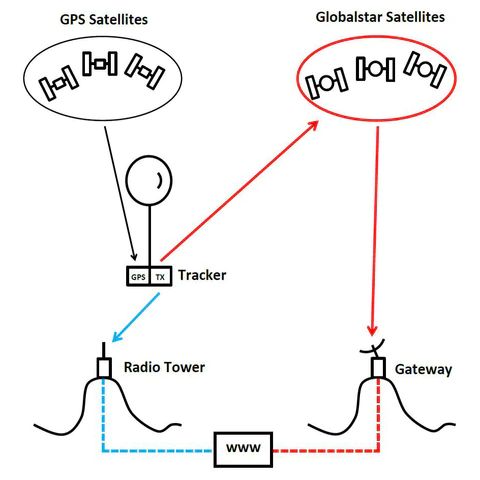
\includegraphics[width=0.3\textwidth]{gps_relay}
  \caption{GPS Relay Tracking \cite{site-highaltitudescienceTrackingWeather}}
  \label{fig:gps_relay}
\end{figure}

The major disadvantage of this method is the additional cost required. Since an antenna capable of communicating with one of the external networks is required, two antennas are needed if direct communication with a ground station is desired (however this is usually no longer necessary as the relay network can be used). Further, the cost of subscribing to an external network is generally high.

This type of tracking works well if the satellite is physically close to the external network satellites, or if the ground station does not need to communicate in real-time, but merely needs access to the location of the satellite e.g. in a home-made balloon satellite launch.

\subsection{Signal Strength}
Radio tracking can be done when the satellite itself transmits omni-directionally. The received signal strength can be used as feedback to determine the direction to point. To initially find the satellite, the entire sky can be scanned using a "brute force" procedure, or an initial guess can be provided. Then, periodic \textit{radius scanning} can be used to track the signal within a certain portion of the sky, or more advanced techniques such as \textit{conical scanning} can be used, to calculate a new direction to point given a set of conically signal strength measurements.

This method provides great flexibility, since no satellite path information is required, however it is generally not necessary when a reasonable initial guess is available, and an antenna with a reasonably large beamwidth is used.